\section{实验}
\label{sec:tabel-eval}


本节中,我们首先介绍用于实验的跨语言表格链接数据集,
以及已有的基线方法,这些方法主要是由单一语言上的实体链接方法转换而来。
我们在跨语言以及单一语言场景下进行了端到端测试,
并且通过横向对比实验分析方法中不同模块的重要性。


\subsection{实验设置}
\label{sec:tabel-exp-setup}


%In this section, we introduce how we perform word embedding on Wikipedia,
%and how the cross-lingual table linking dataset is constructed.

\textbf{词向量、实体向量学习:}
我们使用2017年2月版本的中文与英文维基百科\footnote{
\url{https://dumps.wikimedia.org/zhwiki/},以及\url{https://dumps.wikimedia.org/enwiki/}。
}语料库,用于学习模型中的词向量与实体向量。
语料库中包含5,346,897个英文实体以及919,696个中文实体。
为了学习每个实体向量,
我们将维基百科中的锚文本替代为一个特殊词语,与背后的实体一一对应。
例如英文句子 ``the \underline{Rockets} All-Star player James Harden ... '' 中,
锚文本 ``Rockets'' 对应的实体为 ``Houston Rockets'' ,
因此我们使用与之对应的特殊词语 ``[[Houston\_Rockets]]'' 替代锚文本。
这样处理的好处在于,实体和普通词语之间无差别,
英文的词汇和实体用同一连续语义空间进行表达,
这也使得模型经过翻译层后,更容易捕捉字面描述与实体间的相关性。
预训练过程采用Word2Vec\parencite{mikolov2013distributed}分别学习中文和英文语料库上的词向量,
特殊词语向量即为对应实体向量。
预训练的词向量维度设为100。
%The advantage is that,
%by learning embeddings of both common and special words in a uniform vector space,
%each entity can be represented by the embedding of its identical word,
%which is more precise than the aggregation of word embeddings in the entity's name.
%Besides, in order to enlarge the number of anchor texts in the corpora,
%we automatically add more anchor texts to both Chinese and English Wikipedia:
%for each article page, we simply find all the surface form of phrases exactly matching the article name,
%and then transform these phrases into an anchor text, linking to the current article.

\textbf{表格链接数据集:}
%since cross-lingual table linking is a new task, we do not have any existing benchmarks,
%and we have to construct a dataset by ourselves.
%Our cross-lingual table linking dataset consists of 150 web tables with
用于实验的跨语言表格数据集包含150个中文字面描述的互联网表格,
以及对应的链接表格,标注的实体来自于英文维基百科。
大部分表格来自Wu等人的研究\parencite{wu2016entity},
其公布的数据集包含123张中文表格,以及映射到中文维基百科上的实体。
我们在互联网中收集了另外40张大小相似的中文表格,
再利用维基百科的跨语言链接以及人工标注,生成所有的英文链接表格。
大约81\%的单元格可以找到对应的英文实体。
我们过滤掉表格过小,或可被链接的单元格过少的表格。
最终数据集包含150张表格,共有3,818个单元格,其中2,883个单元格标注了链接实体,
平均每张表格包含19.22个链接实体。
%if the shape is smaller than 5*3, 
%or if the number of labeled English entities is smaller than its columns.
%The whole dataset comes from 2 sources. We collect xx tables from Wutianxing \shortcite{},
%and construct the remaining xx tables by human annotation: among xxx tables extracted from
%Chinese Wiki dataset, we randomly sample xx tables with at least x rows and x columns.
%For each cell in the table, if it should be linked to a Chinese Wiki page
%but the link is missing in the original table, we manually add the link to this cell.
%This work is done by x annotators in x hours.
%Then we transform all the Chinese concepts into English concepts via inter-language links in Wikipedia.
我们将数据集随机分为训练集、验证集和测试集,比例为80:20:50。
%TODO: https://adapt.seiee.sjtu.edu.cn/tabel


\subsection{基线模型}
\label{exp:tabel-soat}

由于之前并没有直接针对于跨语言场景的表格链接工作,
因此我们从两个角度出发,根据已有工作构建用于比较的模型。

第一个方向是单语言的表格链接系统,
我们主要关注Bhagavatula等人\cite{bhagavatula2015tabel}
以及Wu等人\cite{wu2016entity}的工作。
这两个系统分别在英文表格链接与中文表格链接上取得了不错的结果,
分别简写为$TabEL_B$以及$TabEL_W$。
为了使这两个系统能在跨语言场景中进行测试,
我们通过单一翻译工具将输入中文表格转换为英文,
这样整个实验变成了单语言的场景,两个系统可以直接运行。

第二个方向是跨语言的实体链接系统,
我们与Zhang等人\cite{zhang2013cross}的工作进行比较,
简写为$TextEL$。
该方法对LDA主题模型\cite{blei2003latent}进行改进,称为双语LDA模型。
其核心在于同一个隐含主题具有两个不同语言上的词汇概率分布,
通过比较字面描述上下文与候选实体在主题概率分布上的相似度,
确定最佳的链接结果。
%This work aims at entity linking from foreign languages to English on unstructured texts,
%and authors proposed the BLDA model, which models each foreign text and English Wiki article
%as the probabilistic distribution of latent bilingual topics in a uniform space.
为了将该模型用于表格上的实体链接,
我们将表格按行遍历方向展开成普通文本,
并标记文本中所有需要被链接的短语位置。
经过此法,$TextEL$可以在文本中捕捉更灵活的上下文信息,
但有可能丢失列方向上实体相关的特性。
%也许可以讲的更细一些

\subsection{实验结果}

\subsubsection{候选实体生成测试}
\label{sec:tabel-exp-cand-gen-eval}

%In this part, we evaluate the quality of candidate entity generation.

本节中,我们关注将中文字面描述翻译为候选实体的精准度。
根据\secref{sec:tabel-impl}中的介绍,我们使用了三种不同的翻译工具用来生成候选实体。
我们通过Hits@$n$指标来衡量候选生成结果的好坏,以比较不同翻译工具带来的差别。
Hits@$n$的定义为正确的英文实体出现在前$n$个候选实体中的单元格比例。
具体比较结果如\tabref{tab:tabel-cand-gen-quality}所示,
从中观察可知,百度翻译的结果稳定优于另外两者,
而当所有翻译工具全部使用时,相比百度翻译结果,
Hits@5和Hits@10都能稳定增长约4\%。
这说明了多个翻译工具之间互相补充,有助于发现更多正确的实体,
同时有效的字面相似度的候选排序避免了过多错误的候选实体被引入。%写的不好
%ensembling multiple translation resources is able to discover more correct entities without bringing too many noisy candidates.

\begin{table}[ht]
    \centering
    \bicaption{候选生成步骤的Hits@$n$测评结果。}{Hits@$n$ results on candidate entity generation.}
    \begin{tabular} {c|ccc}
        \hline
        Resources    &   n=1     &   n=5     &   n=10    \\
        \hline
        Baidu      &   0.542   &   0.669   &   0.684   \\
        Google     &   0.463   &   0.585   &   0.596   \\
        Tencent    &   0.394   &   0.510   &   0.522   \\
        \hline
        All Used    & \textbf{0.558}  & \textbf{0.708}  &  \textbf{0.726}   \\
        \hline
    \end{tabular}
    \label{tab:tabel-cand-gen-quality}
\end{table}



\subsubsection{端到端测试}
\label{sec:tabel-exp-e2e-results}

%1. overview & metric (3 sents)
本节中,我们将与其它基线模型$TabEL_B$,$TabEL_W$和$TextEL$在跨语言场景上进行端到端测试。
与已有工作的实验保持一致,我们使用的评价指标为
微观准确率(Micro Accuracy)和宏观准确率(Macro Accuracy)。
微观准确率统计所有测试表格中,实体链接正确的单元格比例,
而宏观准确率定义为每个表格各自链接准确率的平均值,避免了评价指标倾向于更大的表格。

%In order to keep a fair comparison,
由于$TabEL_B$和$TabEL_W$仅通过一种翻译工具生成输入表格的英文描述,
出于公平考量,我与基线模型的比较实验均仅使用百度翻译。
与此同时,我们也评估使用所有翻译工具,并且进行预训练的模型准确率。
基于测试集上微观准确率的调参,我们使用的模型超参数为
$N_{cand}=30$,$N_{tab}=49$,$d_{cell}=d_{cont}=100$,$d_{out}=200$,$\eta=0.0002$以及$p=0.9$。
%For other approaches, we use different $N_{cand}$, tuning separately.

\tabref{tab:tabel-main-result}显示了端到端实验的比较结果。
首先关注上面四行仅使用百度翻译的实验,
我们模型的大幅度优于其余基线模型,准确率得到了约12.1\%的相对提升。
在此基础之上,使用多个翻译工具模型将微观准确率提升了0.03,
再次表明翻译工具之间的互补性给整个系统带来的帮助。
双语翻译层的预训练步骤同样具有明显效果,进一步将微观准确率提升了0.023。
基于单语言表格链接模型的$TabEL_B$与$TabEL_W$受困于翻译过程带来的局限性:
实体预测结果严重依赖唯一的英文翻译,一旦出现偏差便很难纠正,整个系统容错率较低。
由于模型的后续训练切断了与原始中文描述之间的联系,
这导致了翻译步骤无法收到训练数据提供的反馈,因此错误只能在模型中传播。
作为对比,我们提出的模型利用多种英文翻译生成大量候选实体,
并将原始中文描述作为输入学习特征表示,尽可能减轻了翻译过程的信息流失。
%作为对比,我们提出的模型对原始中文描述进行编码,
%并通过双语翻译层与英文实体匹配,避免使用可能出错的英文翻译。

\begin{table}[ht]
\centering
\bicaption{跨语言表格链接的测试结果,基线模型仅使用百度翻译工具。}
{Cross-lingual table linking results. All baselines take Baidu as the only translating tool.}
\label{tab:tabel-main-result}
\begin{tabular} {c|c|cc}
    \hline
    Approach          & Micro Acc.   & Macro Acc.    \\
    \hline
    $TabEL_B$         &  0.512       & 0.507         \\
    $TabEL_W$         &  0.514       & 0.519         \\     %N_{cand} = 10
    $TextEL$          &  0.472       & 0.458         \\
    \hline
    Ours (Baidu Only) &  0.576       & 0.573         \\
    Ours (Full, - pre-train) &  0.606    &  0.591        \\ 
    Ours (Full, + pre-train)  &  \textbf{0.629}       & \textbf{0.614}         \\
    \hline
\end{tabular}
\end{table}


接下来,我们进一步分析候选实体数量$N_{cand}$将对模型效果产生怎样的影响。
显而易见的是,一方面随着$N_{cand}$增大,候选实体中包含正确实体的概率也随之增大,
意味着模型准确率的理论上限将会提高,
而另一方面,$N_{cand}$增大会引入更多干扰实体,整个系统也就更难达到理论上限。
我们在不同的模型上改变$N_{cand}$值,进行了多组比较实验,
微观准确率结果如\figref{fig:tabel-trend}所示,
图中标出了微观准确率的理论上限。
%其结果等同于Hits@$n$指标。
我们的方法在不同大小的候选数量上均有良好的适应性,
随着$N_{cand}$增大,一直保持着稳定的效果提升。
$TabEL_B$的效果比较稳定,但带有微小的准确率下降。
而$TextEL$结果出现了急剧下降,拐点位置的候选数量甚至没有超过10。
我们认为主要原因在于双语LDA模型基于无监督学习方式,
它没有获得任何直接的\textless 中文描述,英文实体 \textgreater 信息用于训练,
因此对干扰实体的数量非常敏感。
%Two main reasons are:
%1) the BLDA model is unsupervised, though equivalent articles between
%Chinese and English Wikipedia pair together as the input documents, the model doesn't observe
%any explicit (mention, entity) pair for learning,
%2) the similarity between the mention and the entity is only determined by their topic
%distributions, without features derived from entity names, or from coherence information.
%These reasons make $TextEL$ much more sensitive to noisy candidates.

%with less error propagation during the translation step,


\begin{figure}[th]
\centering
\includegraphics[width=0.9\columnwidth]{figure/tabel/main-result-crop.eps}}
\bicaption{微观准确率随候选实体数量$N_{cand}$的变化情况。}{Results of Micro Accuracy by different size of candidates.}
\label{fig:tabel-trend}
\end{figure}




为了更好地证明模型的有效性,我们对单语言场景的表格链接也进行了测试。
由于跨语言的数据集利用中英文维基百科之间的链接构建,
因此只需把标注实体替换为对应中文维基实体即可。
相应地,我们从模型中移除双语翻译层,并保持其余设置不变。
用于比较的系统依然为$TabEL_B$和$TabEL_W$,
两者均为表格链接的代表工作,其中后者为中文表格链接任务的最好结果。
\tabref{tab:tabel-mono-result}列出的实验结果显示,
我们模型的单语言版本依然优于两个基线系统,
这在一定程度上说明了基于神经网络的联合训练模型的有效性,
可以从表格的行列之中捕捉有意义的语义信息。

\begin{table}[ht]
	\centering
	\bicaption{中文环境下的表格链接准确率。}{Accuracies on Chinese mono-lingual table linking.}
	\label{tab:tabel-mono-result}
	\begin{tabular} {c|c|cc}
        \hline
		Approach          & Micro Acc.   & Macro Acc.    \\
		\hline
		$TabEL_B$         &  0.848       & 0.845         \\
		$TabEL_W$         &  0.852       & 0.848         \\     
		Ours-mono  &  \textbf{0.886}       & \textbf{0.868}   \\
        \hline
	\end{tabular}
\end{table}





\subsection{模型分析测试}
\label{sec:tabel-ablation}

本节中,我们对提出的神经网络模型进行了更加详细的实验分析,
探索模型中指示、上下文、一致性特征各自的贡献程度,
以及联合训练的模型架构所带来的优势。

\subsubsection{三类特征的作用}

为了研究模型涉及到的三种不同特征的贡献程度,
我们使用不同的特征组合,在跨语言场景中进行对比测试。
比较结果如\tabref{tab:tabel-ablation-features}所示,
模型中的每一类特征都对最终的准确率起到积极贡献。
其中,指示特征是最重要的特征,
因为它提供了字面描述与目标实体之间最为直接的信息。
上下文特征的作用也十分明显,在维基百科中,
实体对应的锚文本周围很可能出现与其同行或同列的其它描述,
因此基于CBOW或Skip-Gram训练的实体向量包含这些上下文的语义。
我们观察到,如果仅使用一致性特征进行训练,
准确率的降低十分明显,约为59.6\%,
这主要是因为模型难以获取实体与字面描述之间,
最主导和直接的语义关联。
但这并不影响一致性特征对指示及上下文特征的补充,
若去除该特征,模型准确率将相对下降约6\%,依然是不小的差距。
一致性特征旨在从全局角度发现实体之间的潜在关联,
用来表征同一列实体之间是否具有一致性,例如隶属于相同的维基百科分类标签。
即便模型没有直接利用每个实体的分类标签信息,
一致性特征依然可以在向量表示中寻找依据。

\begin{table}[ht]
	\centering
	\bicaption{不同特征组合在验证集上的跨语言链接准确率。}{Ablation test of feature combinations on validation set.}
	\label{tab:tabel-ablation-features}
	\begin{tabular} {c|c|c}
        \hline
		Feature Combination &   Micro Acc.  & Decrease in Acc. (\%) \\
		\hline
		Mention Only           &   0.604    & 12.7 \\
		Context Only        &   0.576    & 16.7   \\
		Coherence Only      &   0.279    & 59.6     \\
		Mention + Context      &   0.652    & 5.78    \\
		\hline
		Full                &   0.692    & 0.00  \\
        \hline
	\end{tabular}
\end{table}

我们用本章开头的\figref{fig:tabel-intro}举例讨论一致性特征的有效性。
第三列中字面描述 ``{钢铁侠}'' 具有很高的歧义,
在维基百科中,它可以对应超级英雄 ``Iron\_Man'' ,也可以对应电影 ``Iron\_Man\_(2008\_film)'' 。
作为对比, ``{驯龙高手}'' ( ``How\_to\_Train\_Your\_Dragon\_(film)'' )以及
``{线人}''  ( ``The\_Stool\_Pigeon\_(2010\_film)'' )相对来说歧义较小。
若只使用指示特征和上下文特征,模型预测的实体为超级英雄,
考虑到钢铁侠在更多文本中确实代表超级英雄,
因此这样的预测结果可以理解,但却是错误的。
当一致性特征引入之后,联系其它两个歧义较低的实体,
同一列实体之间强烈的相关性使得模型倾向于这一列都预测电影,
因此模型能够实现正确的预测。


% \begin{figure}[th]
% \centering
% %\epsfig{file=fb-schema-4.eps, width=0.95\columnwidth}
% \scalebox{0.25}{\includegraphics[angle=0]{figures/example.eps}}
% \caption{A real example of table linking. The red arrow points to the entity 
% predicted without using coherence feature, and the green arrow points to the entity
% predicted by using all features.}
% \label{fig:example}
% \end{figure}


\subsubsection{联合模型的作用}

这部分将验证整个联合模型框架的作用。
相对于联合模型计算整个输入表格与链接表格的相关度,
非联合模型中,单元格之间完全独立,各自计算字面描述与候选实体的匹配程度,
最后求平均得到整张表格上的相关度。
%受Sun等人\parencite{sun2015modeling}工作的启发,
我们将联合模型进行退化,
由于非联合模型仅考虑单个单元格,我们移除模型中的一致性特征模块,
并无需对不同单元格的特征输出求平均。
%Add formula if possible.
%which maximizes the margin between the gold entity $e^+$ and
%all the negative entities $e^-$ of the mention $x$.
%We investigate the effect of joint model without introducing the coherence feature.
%As discussed before, the cell and context features focus on relationships of individual mentions,
%then we simply transform the table linking problem into a traditional entity linking problem.
%%:given a mention's cell and context embedding (rather than a table of multiple mentions),link the mention to an entity in the knowledge base.Also, the gold linking result of a training table becomes a list of $(mention, entity)$ pairs.
%
%In this model,  $score(\cdot, \cdot)$ is similar with \eqnref{eqn:score},
%but remove the coherence feature, and don't need to average cell and context features over mentions.
%The parameter $\lambda$ is tuned in \{1.0, 2.0, 3.0, 4.0\}.
作为对比实验,我们同样从已有的联合模型中移除一致性特征,
并尝试分别使用RankNet模型或最大间隔损失(Max Margin)进行训练。

\begin{table}[ht]
    \centering
	\bicaption{不同模型训练方式在测试集上的跨语言链接准确率。}
    {Ablation test of train strategiess on validation set.}
    \label{tab:ablation-joint}
    \begin{tabular} {c|c|c|c}
        \hline
        Model       & Optimizer     & Coherence  &  Micro Acc.   \\
        \hline
        Non-Joint   & Max Margin    & N     & 0.586         \\
        Joint       & Max Margin    & N     & 0.574         \\
        Joint       & RankNet       & N     & 0.598         \\
        Joint       & RankNet       & Y     & 0.629         \\
        \hline
    \end{tabular}
\end{table}

\tabref{tab:ablation-joint}列出了这一部分实验在测试集上的微观准确率结果。
对比前两行结果,我们可以发现,若使用最大间隔损失,
非联合模型的效果反而优于联合模型。
主要原因有以下两点:
1) 非联合模型中,每一个单元格的多个负样本实体都能在训练过程中被利用,
而对于联合模型,由于负样本表格的生成依靠随机采样,并不是所有的负样本实体都会被使用;
2) 最大间隔损失侧重于正样本表格与不同负样本表格间的分值差距,
而对于不同错误程度的负样本表格之间,它们的偏序关系并没有被有效利用。
因此,相比于最大间隔损失,基于成对计算损失的RankNet更加适合于联合模型。
此外,在算法运行速度方面,非联合模型无需迭代预测步骤,因此显然比联合模型更高效。
而实验过程显示,联合模型平均只需要6轮迭代即可完成对每个测试表格的链接预测,
是一个可以被接受的运行速度。

